\documentclass[12pt,a4paper]{article}
\usepackage[utf8]{inputenc}
\usepackage[T5]{fontenc}
\usepackage[vietnamese]{babel}
\usepackage{hyperref}
\usepackage{graphicx}
\usepackage{listings}
\usepackage{xcolor}
\usepackage{geometry}
\geometry{a4paper, margin=2cm}

\title{\textbf{BÁO CÁO THỰC HÀNH OOP - TUẦN 5}}
\author{\textbf{MSSV:} 202418834 \quad \textbf{Họ tên:} Trần Tuấn Anh}
\date{\today}

\begin{document}
\maketitle

\section{Link Github - Mã nguồn}
Link kho lưu trữ Github chứa mã nguồn: \href{https://github.com/tuananhtran109/OOP-Ex05}{https://github.com/tuananhtran109/OOP-Ex05}

\section{Phân tích yêu cầu nghiệp vụ}
Hệ thống quản lý thiết bị và bảo trì trong phòng thực hành yêu cầu khả năng lưu trữ thông tin chung của các thiết bị (như mã, tên, giá, năm sử dụng) và tính toán chi phí bảo trì tùy theo từng loại thiết bị cụ thể.
\begin{itemize}
    \item \textbf{Quản lý danh sách}: Hệ thống quản lý ba loại thiết bị chính (Máy tính, Máy in, Máy chiếu), mỗi loại có đặc thù riêng về thông số kỹ thuật (RAM/GPU, số trang in, số giờ sáng...).
    \item \textbf{Tính toán phí bảo trì}: Mỗi loại có một công thức tính chi phí bảo trì độc lập dựa trên hao mòn đặc trưng, đòi hỏi thiết kế đa hình.
    \item \textbf{Hỗ trợ mạng}: Có các thiết bị yêu cầu kết nối mạng (toàn bộ máy tính, một phần máy in), yêu cầu hệ thống cung cấp cách truy xuất đồng nhất đối với các thiết bị mạng mà không phụ thuộc vào lớp cụ thể của thiết bị.
    \item \textbf{Phân bổ}: Các thiết bị được phân bổ vào các phòng (LabRoom). Thiết bị có thể tồn tại độc lập với phòng (quan hệ Kết tập / Aggregation).
\end{itemize}

\section{Danh sách lớp và sơ đồ quan hệ}

\begin{center}
    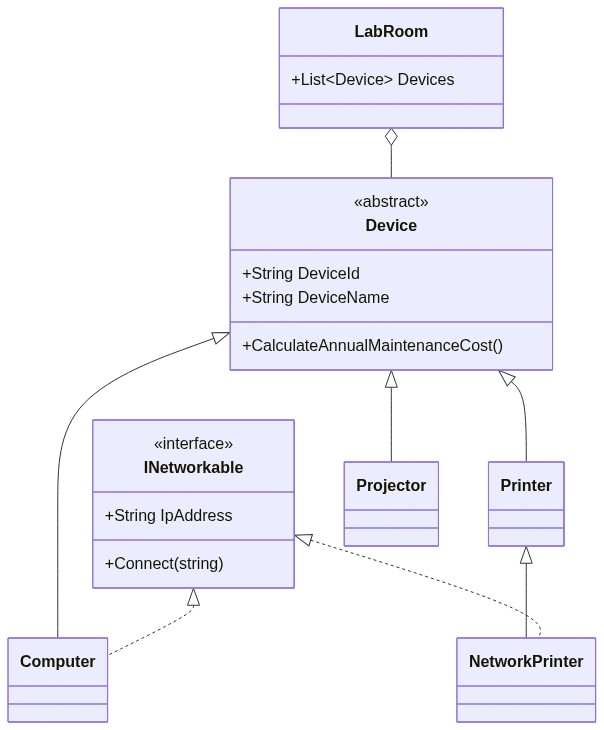
\includegraphics[width=0.9\textwidth]{diagram.png}
    
    \textit{Sơ đồ lớp (Class Diagram) của hệ thống}
\end{center}

\textbf{Danh sách các lớp / giao diện:}
\begin{itemize}
    \item \texttt{Device} (abstract class): Lớp cơ sở trừu tượng đại diện cho mọi thiết bị.
    \item \texttt{Computer}: Lớp dẫn xuất từ \texttt{Device}, thực thi \texttt{INetworkable}.
    \item \texttt{Printer}: Lớp dẫn xuất từ \texttt{Device}.
    \item \texttt{NetworkPrinter}: Lớp dẫn xuất từ \texttt{Printer}, thực thi \texttt{INetworkable} (Tách riêng để thiết kế mạng linh hoạt, thỏa mãn nguyên lý Liskov Substitution).
    \item \texttt{Projector}: Lớp dẫn xuất từ \texttt{Device}.
    \item \texttt{LabRoom}: Lớp đại diện phòng máy, chứa danh sách \texttt{Device}.
    \item \texttt{INetworkable} (interface): Giao diện mô tả khả năng kết nối mạng.
    \item \texttt{DeviceStatus}, \texttt{PrinterType} (enum): Trạng thái thiết bị và loại máy in.
\end{itemize}

\textbf{Quan hệ giữa LabRoom và Device:}
Quan hệ giữa \texttt{LabRoom} và \texttt{Device} là quan hệ \textbf{Kết tập (Aggregation)}. Do theo nghiệp vụ, "Thiết bị vẫn có thể tồn tại trong hệ thống khi chưa được phân bổ vào phòng nào". Nếu phòng thực hành (\texttt{LabRoom}) bị xóa hoặc dỡ bỏ, các đối tượng \texttt{Device} vẫn tồn tại và có thể được phân bổ sang phòng khác, nghĩa là vòng đời của chúng hoàn toàn độc lập với nhau.

\section{Kết quả chạy}

\subsection*{1. Thêm thiết bị vào phòng}
\begin{center}
    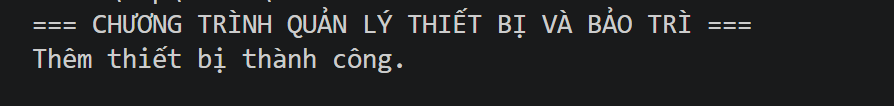
\includegraphics[width=0.8\textwidth]{kq1.png}
\end{center}

\subsection*{2. Thử thêm một thiết bị bị trùng mã}
\begin{center}
    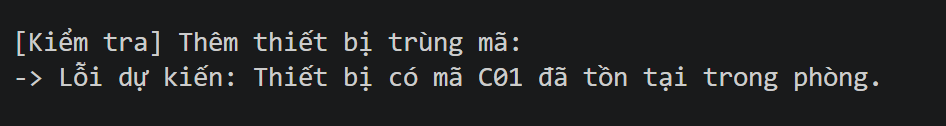
\includegraphics[width=0.8\textwidth]{kq2.png}
\end{center}

\subsection*{3. In danh sách thiết bị trong từng phòng}
\begin{center}
    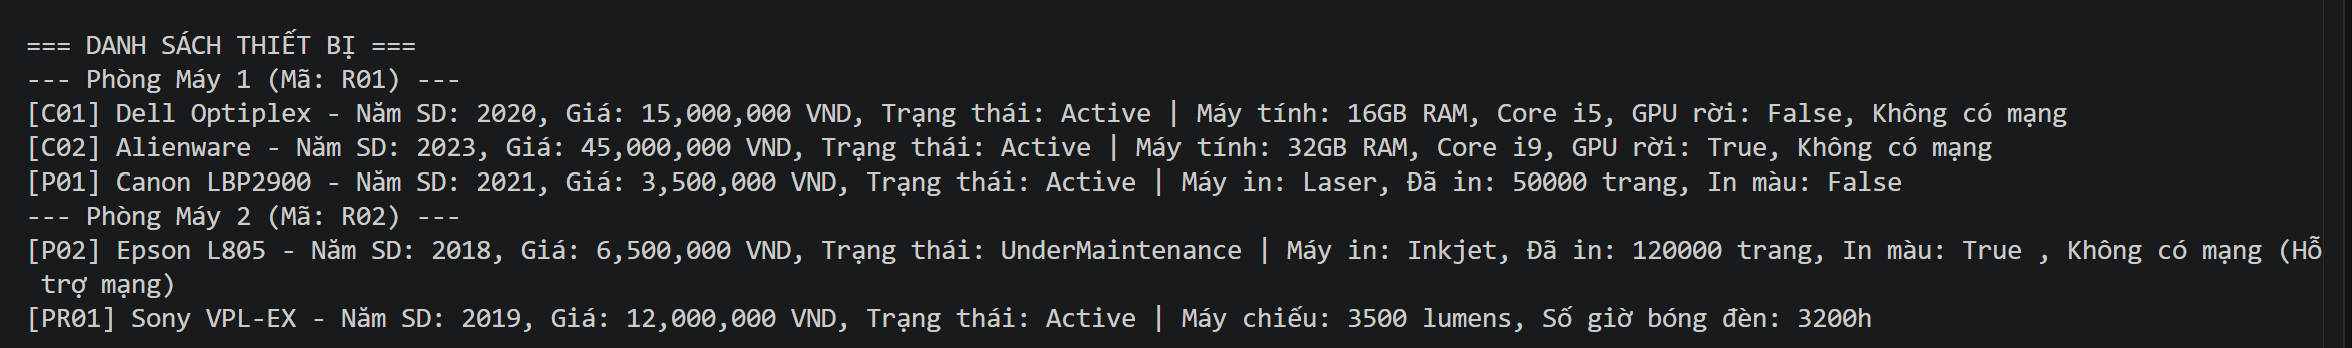
\includegraphics[width=0.9\textwidth]{kq3.png}
\end{center}

\subsection*{4. Tính tổng chi phí bảo trì dự kiến của mỗi phòng}
\begin{center}
    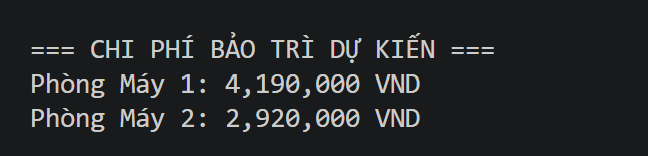
\includegraphics[width=0.8\textwidth]{kq4.png}
\end{center}

\subsection*{5. Liệt kê thiết bị cần bảo trì}
\begin{center}
    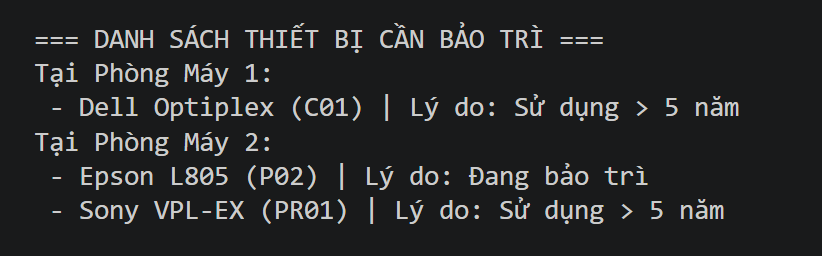
\includegraphics[width=0.8\textwidth]{kq5.png}
\end{center}

\subsection*{6. Kết nối mạng cho các đối tượng thực thi INetworkable}
\begin{center}
    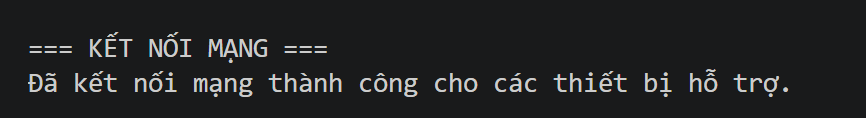
\includegraphics[width=0.8\textwidth]{kq6.png}
\end{center}

\subsection*{7. Duyệt các thiết bị mạng thông qua kiểu INetworkable, không phụ thuộc vào lớp cụ thể}
\begin{center}
    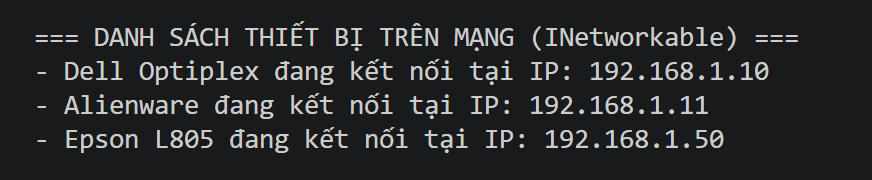
\includegraphics[width=0.8\textwidth]{kq7.png}
\end{center}

\section{Trả lời câu hỏi lý thuyết}
\subsection{1. Vì sao Device là lớp trừu tượng?}
Lớp \texttt{Device} được thiết kế là lớp trừu tượng vì:
\begin{itemize}
    \item \textbf{Không có ý nghĩa khi khởi tạo trực tiếp}: Trong thực tế, không có một "thiết bị chung chung" nào tồn tại, mà phải là một thiết bị cụ thể (Máy tính, Máy in...). Việc ngăn chặn khởi tạo đối tượng \texttt{Device} bằng từ khóa \texttt{abstract} giúp đảm bảo tính hợp lệ của dữ liệu.
    \item \textbf{Định nghĩa khung mẫu (Template)}: Nó đóng vai trò định nghĩa các thuộc tính và hành vi chung mà mọi thiết bị phải có. Đặc biệt, cung cấp phương thức \texttt{abstract CalculateAnnualMaintenanceCost()}, bắt buộc tất cả các lớp con phải tự cung cấp công thức tính phí bảo trì riêng biệt theo đặc thù của mình.
\end{itemize}

\subsection{2. Vì sao INetworkable là interface?}
\texttt{INetworkable} là interface vì:
\begin{itemize}
    \item Khả năng kết nối mạng là một \textbf{năng lực (capability)} được bổ sung thêm chứ không phải là bản chất (không phải quan hệ "is-a" lõi). Do trong C\# chỉ hỗ trợ đa kế thừa đối với interface, việc dùng interface cho phép một lớp như \texttt{Computer} vừa kế thừa bản chất từ \texttt{Device}, vừa bổ sung được năng lực \texttt{INetworkable}.
    \item Việc sử dụng interface giúp \textbf{nhóm các đối tượng theo năng lực}: Hệ thống có thể duyệt qua bất kỳ đối tượng nào (Máy tính, hay một Máy in mạng) có khả năng kết nối và gọi hàm \texttt{Connect} mà không cần biết chúng là loại máy móc gì, giúp giảm bớt sự phụ thuộc vào cây kế thừa thiết bị.
\end{itemize}

\subsection{3. Tính đa hình được thể hiện ở đâu?}
Tính đa hình được thể hiện rõ ràng nhất tại \textbf{phương thức tính toán chi phí bảo trì} trong \texttt{LabRoom}:
\begin{verbatim}
public decimal CalculateAnnualMaintenanceCost() {
    decimal totalCost = 0;
    foreach (var device in Devices) {
        totalCost += device.CalculateAnnualMaintenanceCost(); // <-- ĐA HÌNH
    }
    return totalCost;
}
\end{verbatim}
Khi duyệt danh sách \texttt{Devices} (chứa lẫn lộn Computer, Printer, Projector), chương trình không cần dùng \texttt{if} hay \texttt{switch} để kiểm tra kiểu đối tượng. Thay vào đó, nó gọi chung hàm \texttt{CalculateAnnualMaintenanceCost()}. Tại thời điểm chạy (runtime), hệ thống sẽ tự động liên kết (dynamic binding) và gọi đúng phiên bản phương thức tính chi phí đã được ghi đè (override) trong từng lớp dẫn xuất tương ứng.

Ngoài ra đa hình còn thể hiện ở hàm \texttt{ToString()} khi hiển thị thông tin chi tiết từng đối tượng, và ở việc duyệt tập hợp các thiết bị dưới góc nhìn của giao diện \texttt{INetworkable}.

\end{document}
